\chapter{Implementation}
\label{chap:implementation}

% Editorial revision against 2be212a11ceee7453d2f8beebc04337d3690d117.
% Reconciled with the shared-core interfaces introduced in 71e3e71.
% This text describes the existing ordinary-list implementation, not a completed
% efficient backend. Historical claim audits retain their original identity.

\section{Implementation Scope and Versions}
\label{sec:implementation-scope}
\label{sec:implementation-versions}

The code separates an oracle-backed reference pipeline from the ordinary-list
reconstruction of \textcite{fung1990simplified}. The reference function
\texttt{simplified\_jordan\_sort} certifies the input, constructs family trees,
statistics and a trace, and returns the oracle's sorted output. In contrast,
\texttt{paper\_jordan\_sort\_valid} executes the reconstructed algorithm and
returns \texttt{state.partial\_order.to\_list()}. Its core does not use the
oracle's output or a global rank map. It assumes a pre-certified valid Jordan
sequence with distinct, mutually comparable values.

This chapter describes the revised ordinary-list implementation without
rollback. The pilot and formal timings in \cref{chap:results} belong to an
earlier rollback-enabled version. Removing recovery backups and exception
handlers did not remove split planning, list construction, ownership updates
or local checks. Those historical timings therefore measure neither the
current implementation nor a causal benefit of removing rollback. Source
bindings are retained in \cref{sec:appendix-revision-bindings}.

\Cref{chap:algorithm} specifies initialization, both orientations of
Step~1/2/3, and the executable anchor clarifications. This chapter describes
how the code represents and maintains that state, rather than repeating the
algorithm's rules. The efficient finger-search backend remains to be
implemented and validated; it is not an achieved contribution of the version
described here.

\section{Data Representation}
\label{sec:implementation-input-model}
\label{sec:implementation-state}

An immutable \texttt{PointRef(paper\_index, value)} separates one-based paper
identity from a point's comparable value. A \texttt{PairRecord} retains curve
endpoint IDs and family membership; geometric endpoints are obtained by
comparing their values. The distinction and its consequences for output
anchors are specified in \cref{sec:algorithm-geometric-anchor}.

\texttt{PaperJordanState} holds these records, the processed-prefix length,
the partial order, the end-index-to-pair mapping, the sibling backend and two
family roots. It also holds a fixed execution policy, optional trace and
counters, and mandatory stage results. Sorting and diagnostics use the same
runner and mirrored orientation branches.

\subsection{Partial Sorted Order}
\label{sec:implementation-partial-order}

\texttt{SortedOrderList} is doubly linked, with identity-based infinity
sentinels and a point-ID-to-node mapping. Neighbor access and insertion use
local links. Before mutation, insertion checks that the value lies strictly
between its adjacent values. Final traversal excludes the sentinels and
returns the original values. Mapping access uses Python dictionaries; its
cost must not be silently treated as a deterministic worst-case constant.

\subsection{Sibling Lists and Ownership}
\label{sec:implementation-sibling-lists}

Each \texttt{SiblingList} stores ordered finite pair IDs and one owner.
A pair caches its parent and containing-list IDs, together with its ordered
child-list IDs. Every owned finite pair occurs in exactly one live list,
whose owner equals its parent. A parent has at most two ordered child lists;
finite parent chains must reach the same-family dummy without cycles.
The family dummies are roots, not finite list items.

The ordinary backend retains this eager representation. Since commit
\texttt{71e3e71}, the shared core
uses boundary-list, owner and extreme-child access interfaces instead of
reading those fields directly. General pair-liveness checks do not require
the pair to be a list endpoint. A replacement must implement these accesses
without reconstructing a full list on the timed path; the interfaces alone
establish neither its implementation nor its operation costs.

\begin{figure}[htbp]
  \centering
  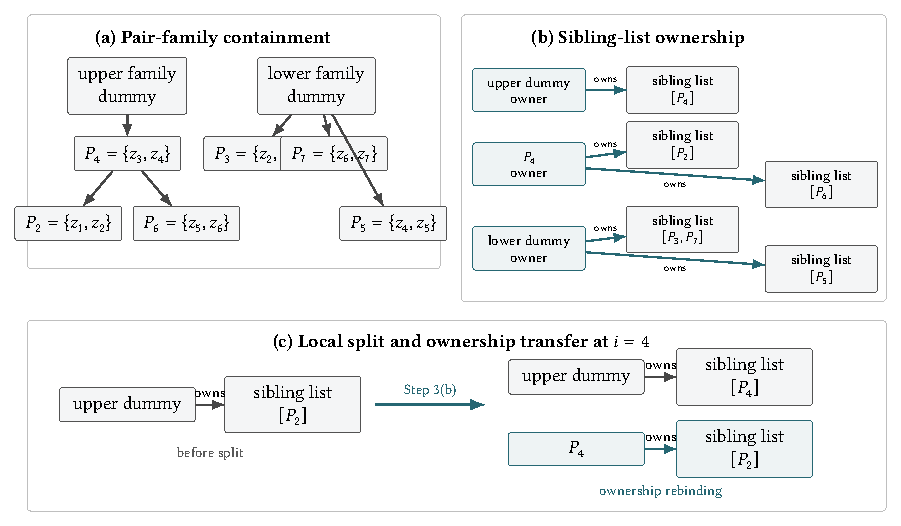
\includegraphics[width=\textwidth]{family_sibling_structure.pdf}
  \caption[Pair families and sibling-list ownership.]{Pair families and
  sibling-list ownership in the example of
  \cref{fig:algorithm-running-example}. Step~3(b) transfers $P_2$ from a
  list owned by the upper dummy to a child list of $P_4$.}
  \label{fig:implementation-family-sibling-structure}
\end{figure}

\section{Core--Backend Interface and Update Semantics}
\label{sec:implementation-control-flow}

\subsection{Initialization, Boundaries and Stage State}
\label{sec:implementation-initialization}
\label{sec:implementation-step1}
\label{sec:implementation-step2}

The initialization in \cref{sec:algorithm-initialization} materializes all
point records but orders only the first three values; shorter inputs use
fixed-size comparisons. Subsequent iterations use the predecessor and
successor boundaries defined in \cref{sec:algorithm-boundary-selection}.
The backend handles singleton creation, boundary insertion, splitting and
ownership transfer; the partial-order structure handles point insertion.

Boundary selections and Step~3 results are stored even with trace disabled.
Later stages consult them to reject incorrect order, repeated stages and
inconsistent parameters. They are execution state, not merely optional
logging. Optional backend-work observations are stored separately from these
mandatory results; complete logical snapshots belong to the audit path.

\subsection{Pair Insertion and Failure Propagation}
\label{sec:implementation-step3a}

For the insertion rules in \cref{sec:algorithm-step3a-increasing,sec:algorithm-step3-decreasing},
the core checks the boundary, registers the new pair and calls singleton
creation or boundary insertion. A later error may leave that registration
in place. The exception propagates; the state is discarded rather than
restored or reused. This contract applies to both orientations.

\subsection{Split Plans and Ownership Transfer}
\label{sec:implementation-step3b}

The ordinary backend implements the partition specified in
\cref{sec:algorithm-step3b-increasing,sec:algorithm-step3-decreasing}
using an immutable \texttt{SplitPlan}. It records the original sequence and
both ordered partitions before mutation. The plan supports stale-plan
rejection, order checks and pair-set conservation; these functions remain
necessary without rollback.

Commit checks the plan and ownership preconditions, prepares nonempty output
lists and affected child slots, retires the input list, publishes the new
lists, and rebinds the pairs. Touched-state postconditions are checked before
success is returned. Rejection covers stale plans, straddling pairs, ownership
mismatches, cycles, unowned parents and a third child list. Errors during
mutation or postcondition checks propagate without restoring earlier state.
Output-list preparation is ordinary update work, not a recovery backup.

\subsection{Point Insertion and Completion}
\label{sec:implementation-step3c}

The backend exposes the relevant extreme child; the core selects its
geometric endpoint and applies the separate odd-index $z_1$ anchor rule of
\cref{sec:algorithm-z1-anchor}. These executable clarifications and their
counterexamples remain in \cref{sec:algorithm-anchor-clarifications}; they
are not attributed to fully explicit wording in the 1990 paper. The partial
order performs the resulting adjacent insertion. Only after it succeeds does
Step~3(c) advance \texttt{processed\_count}.

\section{Certification, Diagnostics and Replay}
\label{sec:implementation-certification}
\label{sec:implementation-validation}

The wrapper \texttt{certified\_paper\_jordan\_sort} runs the oracle and
rejects invalid candidates before entering the pure sorter. Certification is
outside the minimal core's timing scope. An internal exception is propagated
by both sorting and diagnostic entry points: neither retries, returns a
partial output, nor falls back to the oracle or reference pipeline. Output
recovery is reached only after the runner succeeds.

\texttt{paper\_jordan\_diagnostics\_valid} selects \texttt{checked} and audits
initialization and every completed prefix. It checks point identity and
values, partial-order links and order, exact pair membership, ownership and
parent chains, stage records, trace and metrics. Deterministic replay
reconstructs a fresh state using the same core, backend type and immutable
configuration. It compares backend identity, partial order, registries, stage
results, trace, work observations, metrics, and logical and physical snapshots.
Unavailable backends fail explicitly rather than reverting to ordinary lists.
This is same-core state-consistency evidence, not a second independent
algorithm or a replacement for the external sorted-output check.

Failure-injection tests separately check propagation from pair insertion and
split postconditions, including checks retained in \texttt{minimal}.
Public-call tests require one split attempt and no output recovery after
failure. They impose no rollback or failed-state reuse requirement.

\section{Execution Policies and Observation Costs}
\label{sec:implementation-policies}

Five immutable policies control trace recording, selected operation counters
and complete backend validation after split commits. \texttt{checked}
enables all three; \texttt{minimal} disables them. Intermediate policies
isolate observation costs. All use the same Step~1/2/3 sequence and retain
stage results, necessary local checks, input materialization and output
recovery. The revised implementation has no rollback under any policy.

The archived studies instead timed the rollback-enabled implementation,
including recovery-state preparation in \texttt{minimal}; a successful call
need not actually roll back to incur that preparation. The historical scope
is specified in \cref{sec:method-paper-implementation}.

The ordinary backend reports the counters \texttt{split\_items\_scanned} and
\texttt{split\_items\_copied} each add the input-list length once per
successful split. They are logical split-volume measures, not exact
interpreter-level access counts. They omit boundary-insertion copies,
membership scans and repeated validation/materialization passes. Retained
historical counter names do not establish that splits dominate runtime.
Logical volumes, directly observed work and wall-clock timings are therefore
distinct forms of evidence. The shared core accumulates backend-reported
work under an identified metric schema; it does not infer tree copying from
the input-list length.

\section{Actual Costs and Complexity Boundary}
\label{sec:implementation-complexity}

At either boundary, insertion constructs a new Python list containing the
existing IDs and the new pair. Rear insertion is not an in-place
\texttt{list.append()}. Both orientations copy work proportional to the
current sibling-list length. Split additionally scans and partitions the
list, materializes its outputs and rebinds pair ownership.

``Local'' describes the objects a safety check concerns, not constant cost.
The ordinary backend's liveness check uses
\texttt{pair\_ids.count(pair\_id)} for membership,
and backend parent checks scan the containing list at each visited ancestor.
For an ancestor chain $A$, this contributes
$O(\sum_{a\in A}|L(a)|)$, where $L(a)$ contains $a$, rather than a constant
per ancestor. These costs remain in \texttt{minimal}; complete checked
validation and prefix replay add separate untimed work.

The valid increasing input $(1,2,\ldots,2m)$, $m\geq2$, exposes a quadratic
copying lower bound even without split. Starting from one pair per family,
boundary insertions grow the sibling lists to $m$ and $m-1$ while Step~3(b)
skips splitting. The number of existing pair IDs copied is
\begin{equation}
  \sum_{j=1}^{m-1}j+\sum_{j=1}^{m-2}j=(m-1)^2.
  \label{eq:implementation-boundary-copy-lower-bound}
\end{equation}
Thus this input family incurs $\Omega(n^2)$ copying, including in
\texttt{minimal}. This is a source-derived bound on one component of work,
not a curve fit or a tight total bound for all inputs.

The ordinary backend instantiates neither the level-linked structure of
\textcite{hoffmann1986sorting} nor the heterogeneous finger-search structure
of \textcite{fung1990simplified}. An efficient replacement must account for
its search, rebalancing, ownership, metadata and shared-core checks as well as
initialization and output. A fast tree split alone does not establish an
operation bound for the complete update, and none is claimed here for a
backend that has not yet been implemented and validated.
